\documentclass[a4paper,12pt]{report}
\usepackage[utf8]{inputenc}
\usepackage{enumitem} %permite el uso de letras para enumerar
\usepackage{graphicx} %para las imagenes
\usepackage{float} %para fijar las imagenes

\usepackage{tikz}
\usetikzlibrary{arrows.meta, positioning} %para hacer diagramas de bloques

\usepackage[a4paper, %margenes de pagina
  left=2.5cm,
  right=2.5cm,
  top=2cm,
  bottom=2cm,
  includehead
]{geometry}

\usepackage{fancyhdr}
\pagestyle{fancy}
\lhead{UTN-FRC}
\chead{ASyS}
\rhead{2R3}
\cfoot{\thepage}
\setlength{\headwidth}{\textwidth} % Hace que el ancho del encabezado coincida con el ancho del texto
\setlength{\headheight}{15pt}  % Ajusta la altura del encabezado
\setlength{\headsep}{20pt}     % Ajusta la separación entre el encabezado y el contenido

\usepackage{titlesec}
\titleformat{\chapter}[display]
  {\normalfont\Large\bfseries}{}{0pt}{}
\titlespacing*{\chapter}{10pt}{-45pt}{10pt}

\usepackage{etoolbox} 
\makeatletter
\patchcmd{\chapter}{\thispagestyle{plain}}{\thispagestyle{fancy}}{}{} %Muestra encabezado en las paginas con \chapter
\makeatother

\newcommand{\fs}[1]{%
  \par\refstepcounter{section}% Increase section counter
  \sectionmark{#1}% Add section mark (header)
  \addcontentsline{toc}{section}{\protect\numberline{\thechapter.\alph{section}}#1}% Add section to ToC
}
\newcommand{\fss}[1]{%
  \par\refstepcounter{subsection}% Increase subsection counter
  \subsectionmark{#1}% Add subsection mark (header)
  \addcontentsline{toc}{subsection}{\protect\numberline{\alph{subsection}}#1}% Add subsection to ToC
}

\renewcommand{\contentsname}{Tabla de Contenidos}

\title{%
\setlength{\headwidth}{\textwidth} % Hace que el encabezado tenga el mismo ancho que el contenido
\setlength{\headheight}{15pt}  % Ajusta la altura del encabezado
\setlength{\headsep}{10pt}     % Ajusta la separación entre el encabezado y el contenido
  \fontsize{25}{0}\selectfont Universidad Tecnológica Nacional \\
  \fontsize{22}{30}\selectfont Analisis de Señales y Sistemas \\
  \fontsize{20}{25}\selectfont Trabajo Practico 3
}
\author{
Franco Palombo\\
Ignacio Gil\\
Laureano Valentin Reinoso\\
Luciano Tomas Cortesini Perez\\
}
\date{19 / 08 / 2024}

\begin{document}

\maketitle
\tableofcontents
\thispagestyle{plain}

\chapter{Ejercicio 1}
Graficar ambas señales superpuestas, y verificar cuántas muestras de tiempo discreto se corresponden con el rango de
tiempo continuo utilizado para la representación gráfica.

\begin{enumerate}[label=\alph*), left=0pt]
 
  \item \fs{} Una señal analógica $x(t) = e^{-2t} \mu(t)$ se muestrea para generar la secuencia de tiempo discreto 
    $x[n]$, considerar $n = nT_s$, con $T_s = 0.05$, $T_s = 0.01$, $T_s = 0.1$.

    \begin{figure}[H]
      \centering
      \begin{minipage}{0.55\textwidth}
        \centering
        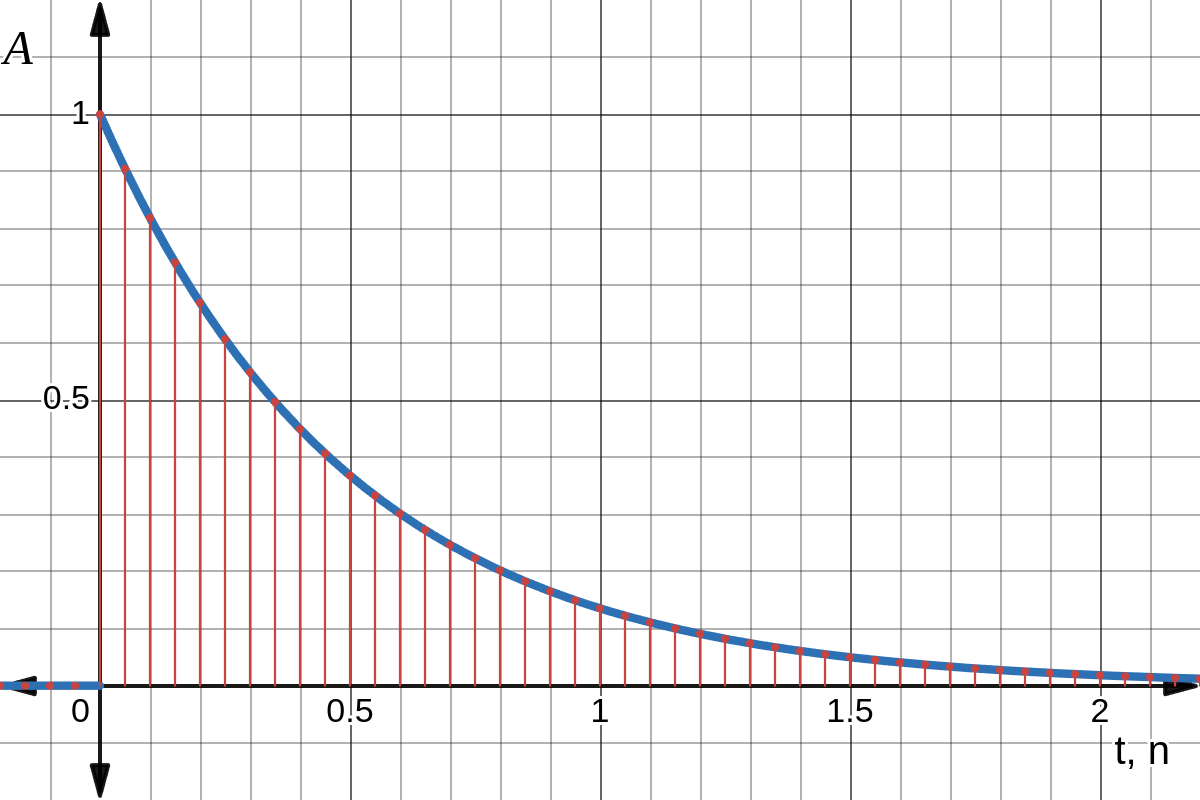
\includegraphics[width=1\textwidth]{./images/ej1.1.png}
        \textit{Muestreo con $T_s=0.05$\\Muestas en el intervalo: $48$}
      \end{minipage}
    \end{figure}

    \begin{figure}[H]
      \centering
      \begin{minipage}{0.55\textwidth}
        \centering
        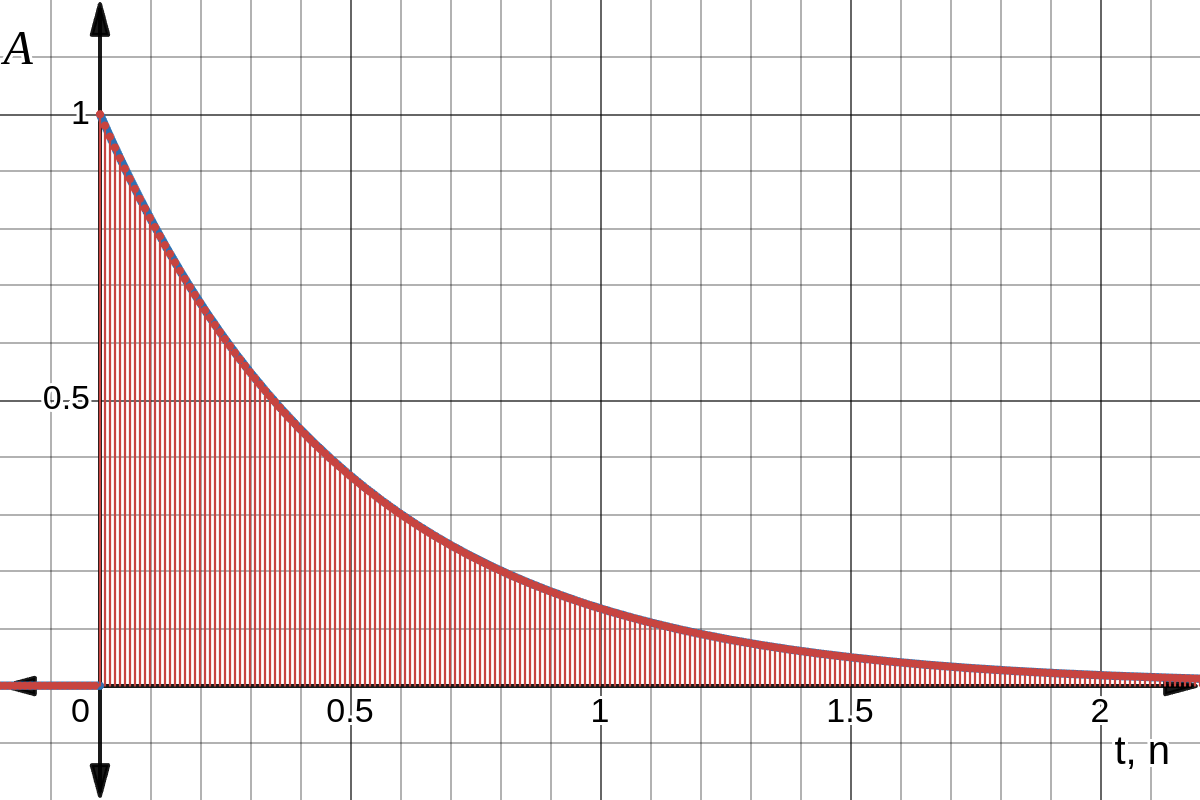
\includegraphics[width=1\textwidth]{./images/ej1.2.png}
        \textit{Muestreo con $T_s=0.01$\\Muestas en el intervalo: $140$}
      \end{minipage}
    \end{figure}

    \begin{figure}[H]
      \centering
      \begin{minipage}{0.55\textwidth}
        \centering
        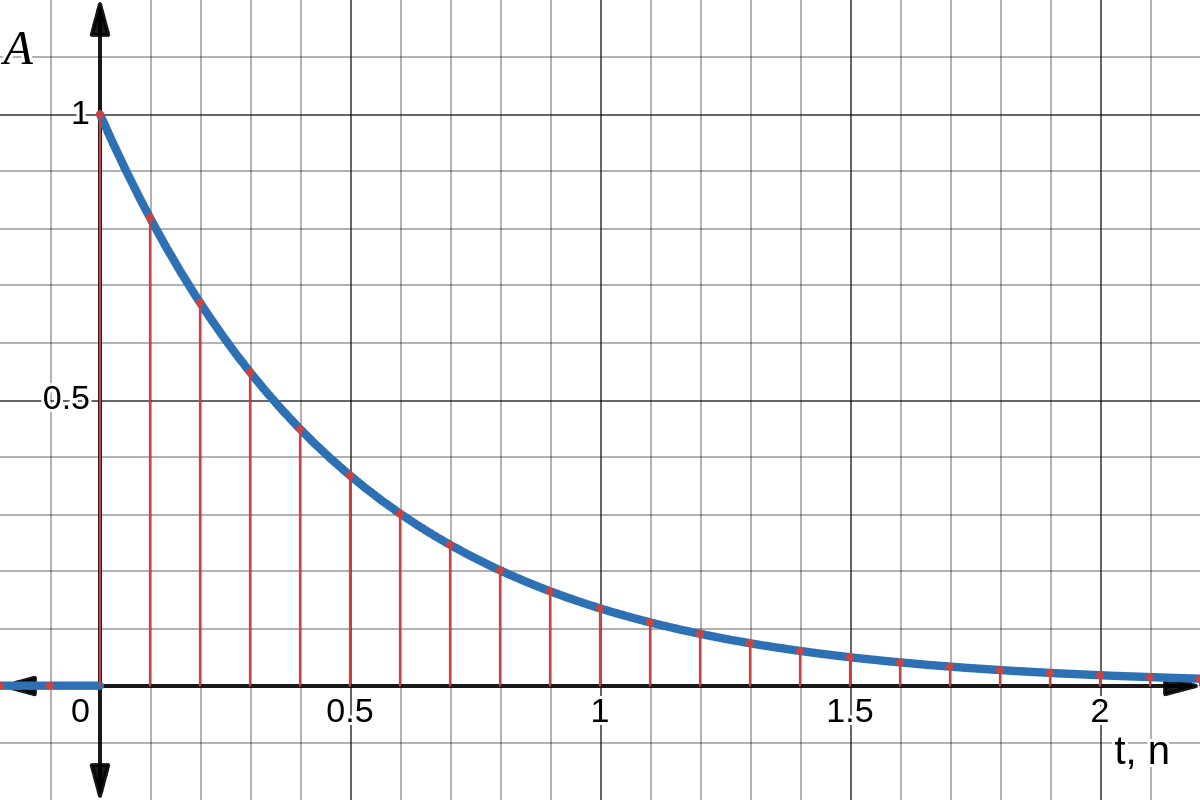
\includegraphics[width=1\textwidth]{./images/ej1.3.png}
        \textit{Muestreo con $T_s=0.1$\\Muestas en el intervalo: $24$}
      \end{minipage}
    \end{figure}


  \item \fs{} Una señal analógica $x(t) = 10 \cos(2t) \mu(t)$ se muestrea para generar la secuencia de tiempo discreto
    $x[n]$, con $T_s = 0.1$ y $T_s = 0.01$.

    \begin{figure}[H]
      \centering
      \begin{minipage}{0.55\textwidth}
        \centering
        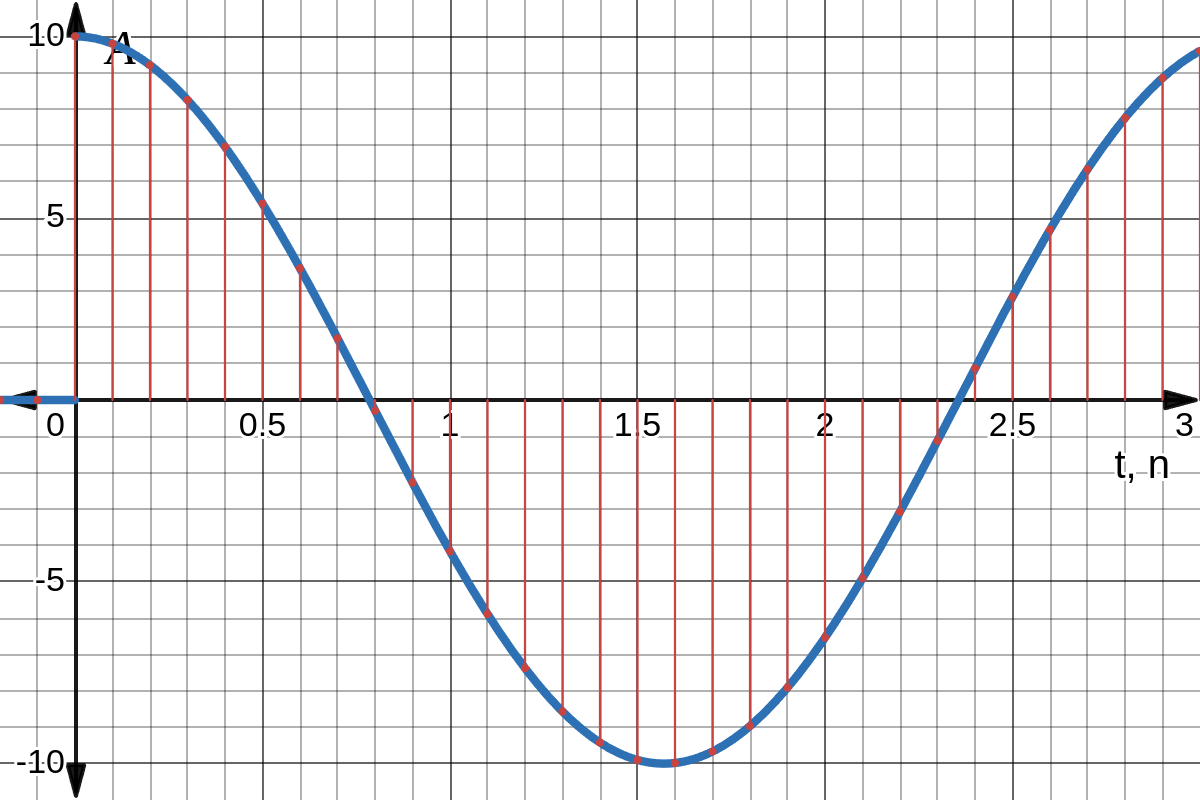
\includegraphics[width=1\textwidth]{./images/ej1.4.png}
        \textit{Muestreo con $T_s=0.1$\\Muestas en el intervalo: $32$}
      \end{minipage}
    \end{figure}

    \begin{figure}[H]
      \centering
      \begin{minipage}{0.55\textwidth}
        \centering
        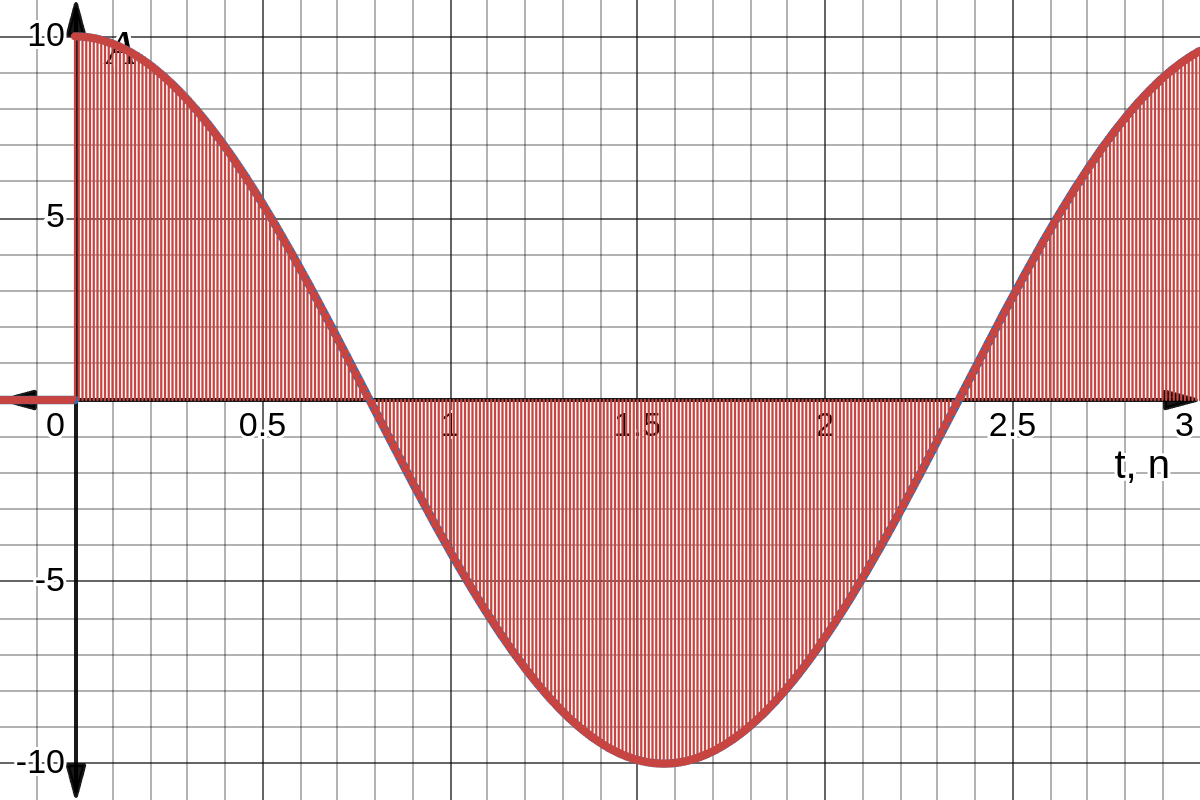
\includegraphics[width=1\textwidth]{./images/ej1.5.png}
        \textit{Muestreo con $T_s=0.01$\\Muestas en el intervalo: $320$}
      \end{minipage}
    \end{figure}

  \item \fs{} Considerar a continuación una secuencia de valores obtenida de una adquisición de datos en un proceso de
    muestreo. Describir una expresión matemática que permita involucrar la secuencia temporal del proceso de adquisición.
    Considerar la secuencia causal:

    \[
    \{0, 3.4, 6, 7, 8.5, 10, 13.4\}
    \]

    Para encontrar una funcion que pase por todos los puntos de la secuencia, como una forma de aproximar la señal en el
    dominio temporal de la cual se obtuvo la secuencia, utilizamos el metodo de interpolación de Lagrange. Definido por:

    $$f(t)= \sum_{j=0}^n f[j] \prod_{i=0,i \neq j}^{n} \frac{t - t_i}{t_k - t_i}$$
    Donde:

    \centering
    \begin{minipage}{0.5\textwidth}
      $n$: número de elementos de la secuencia\\
      $f[k]$: el elemento k-esimo de la secuencia\\
      $t_i$: el instante temporal del elemento i-esimo
    \end{minipage}

    \begin{figure}[H]
      \centering
      \begin{minipage}{0.55\textwidth}
        \centering
        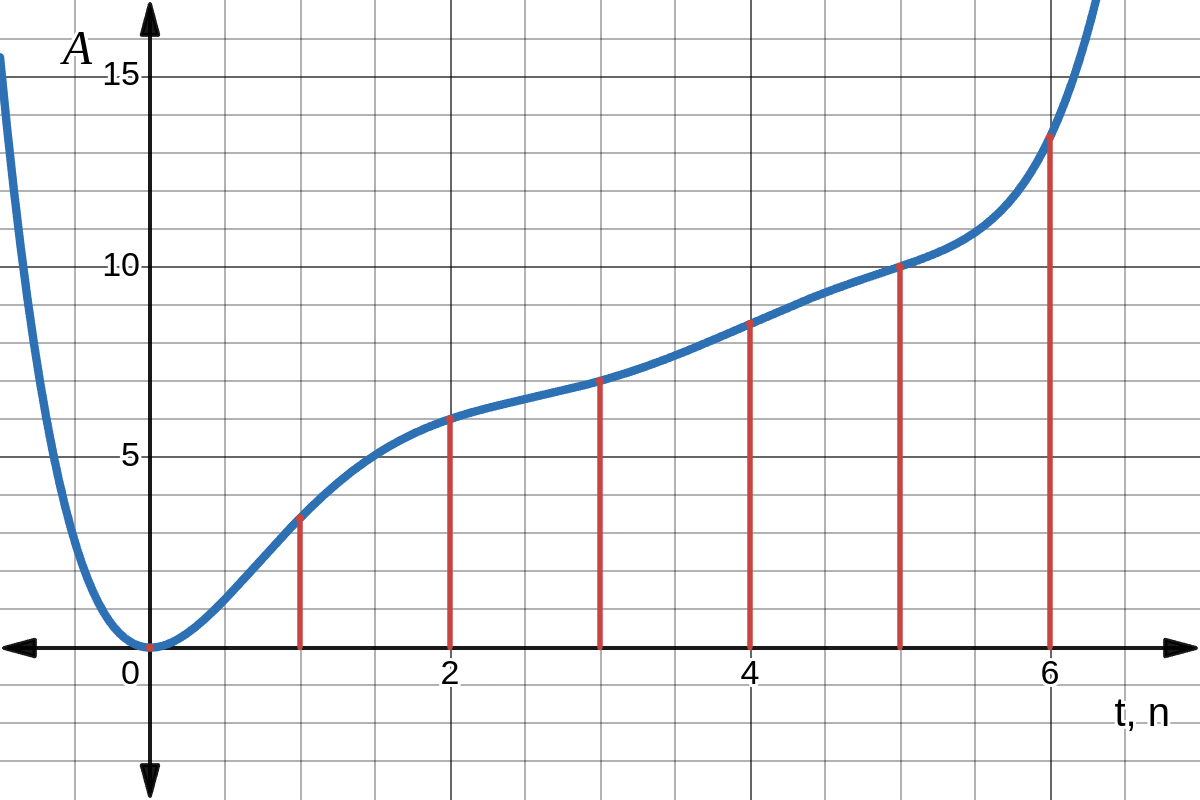
\includegraphics[width=1\textwidth]{./images/ej1.6.png}
        \textit{Interpolación por polinomio de Lagrange}
      \end{minipage}
    \end{figure}

\end{enumerate}

\chapter{Ejercicio 2}
Considerar el siguiente sistema de tiempo discreto:
%Graficar sistema

\begin{enumerate}[label=\alph*), left=0pt]

  \item\fs{} Si $h_1[n] = h_2[n] = 3^{-n}\mu[n]$, $h_3[n] = \mu[n]$, $h_4[n] = 2^{-n}\mu[n]$:

    Calcular la respuesta al impulso del sistema. \\
    Calcular la respuesta del sistema al escalón unitario.

  \item \fs{} Si $h_1[n] = 2^{-n} u[n]$, $h_2[n] = \delta[n]$, $h_3[n] = h_4[n] = 3^{-n} u[n]$:

    Calcular la respuesta al impulso del sistema. \\
    Calcular la respuesta del sistema al escalón unitario.
\end{enumerate}

\chapter{Ejercicio 3}
Considerar un sistema bancario de ahorro a tasa de interés mensual constante. Plantear el sistema considerando un 
depósito mensual constante en el mes $n$ de \$10, $r$ es la tasa de interés en el mismo periodo, y se considera el saldo
inmediatamente después del depósito en el periodo.

\begin{enumerate}[label=\alph*), left=0pt]
  \item \fs{} Identificar en el problema las variables de entrada y salida del mismo.
    % graficar sistema

  \item \fs{} Plantear un modelo en ecuaciones de diferencias capaz de caracterizar el sistema propuesto.

  \item \fs{} Representar la ecuación en diferencias por medio de un diagrama de bloques con retardos unitarios.

  \item \fs{} Evaluar el saldo para un periodo de capitalización de 48 meses.
\end{enumerate}

\chapter{Ejercicio 4}
Considerar este último como la expresión mínima que permita desarrollar un algoritmo de cálculo numérico con la menor
cantidad de operaciones posibles.

\begin{enumerate}[label=\alph*), left=0pt]
  \item \fs{} Diagramar en un diagrama de bloques normalizado representativo del sistema para la siguiente ecuación en
    diferencias:

    \[
    y[n+1] + \frac{1}{2} y[n-1] = x[n] + \frac{1}{2} x[n-1]
    \]

  \begin{tikzpicture}[auto, node distance=2cm, >=latex']

      % Nodes
      \node [input] (input) {$x_n$};
      \node [block] (D) {$D$};
      \node [block] (D2) {$D^2$};
      \node [block] (subtraction) {$\frac{1}{2} x_n - \frac{1}{2} y_n$};
      \node [block] (sum) {\Sum};
      \node [output] (output) {$y_n$};

      % Lines
      \draw [->] (input) -- (sum);
      \draw [->] (output) -- (sum);
      \draw [->] (sum) -- (D2);
      \draw [->] (D2) -- (sum);
      \draw [->] (sum) -- (D);
      \draw [->] (D)--(output);

  \end{tikzpicture}

  \item \fs{} Dado el sistema simulado por el diagrama de bloques a continuación, determinar la ecuación en diferencias
    que lo describe.
    %Graficar sistema

\end{enumerate}

\chapter{Ejercicio 5}
El objetivo de este trabajo práctico es obtener el espectro de frecuencias de una secuencia en tiempo discreto.
Considerar la siguiente secuencia periódica en tiempo discreto y aplicar la Serie de Fourier Discreta (DFT).

\begin{enumerate}[label=\alph*), left=0pt]
  \item \fs{} Obtener el espectro de frecuencias para $N = 3$:

    \[
    x[n] = 1 + \cos \left( \frac{2\pi n}{3} \right)
    \]

    %insertar imagen de la onda muesteada

  \item \fs{} Obtener el espectro de frecuencias para $N = 6$:

    \[
    x[n] = 1 + \cos \left( \frac{\pi n}{3} \right)
    \]

    %insertar imagen de la onda muesteada

\end{enumerate}

\chapter{Ejercicio 6}
Considerar un sistema LTI, causal, caracterizado por una ecuación en diferencias:

\[
y[n] - 1.2 y[n-1] - 0.13 y[n-2] - 0.36 y[n-3] = x[n]
\]

\begin{enumerate}[label=\alph*), left=0pt]
  \item Determinar $Y(z) = \mathcal{Z}\{y[n]\}$, la solución completa, con las siguientes condiciones iniciales:

    \[
    y[-1] = 1, \quad y[-2] = -1, \quad y[-3] = 1
    \]

  \item \fs{} Obtener la función de transferencia $H(z)$, respuesta al impulso con condiciones iniciales nulas, por
    medio de residuos.

  \item \fs{} Obtener $h[n] = \mathcal{Z}^{-1}\{H(z)\}$.

  \item \fs{} Obtener la respuesta al escalón unitario con condiciones iniciales nulas, por medio de fracciones 
    parciales $y[] = \mathcal{Z}^{-1}\{Y(z)\}$.

  \item \fs{} Obtener $y[n] = \mu[n] * h[n]$, la respuesta al escalón unitario sin condiciones iniciales por medio de la
    convolución temporal.

  \item \fs{} Verificar $y[n]$ para la respuesta al escalón unitario por división directa hasta la quinta muestra y
    reconstruir $Y(z) = \mathcal{Z}\{y[n]\}$.

  \item \fs{} Verificar el régimen transitorio (TVI) y el régimen de estado permanente (TVF) en ambos dominios 
    $\{z, n\}$ para la respuesta al escalón unitario con condiciones iniciales nulas.

  \item \fs{} Elaborar la síntesis del sistema por medio de diagrama de bloques con retardos unitarios.
\end{enumerate}

\end{document}

